%----------------------------------------------------------------------
%	CERN TEST BEAM CHAPTER
%----------------------------------------------------------------------
\label{ch:analysis}

Along with verifying the focal plane and radiation hardness of the 3-layer lens design, another crucial step towards solidifying the EIC DIRC design was to test the lens in a prototype DIRC with a real particle beam. Because not all of the components of the high-performance DIRC baseline design for EIC are currently available it is necessary to validate the simulation package currently used to design and optimize the system. In June and July of 2015 the PANDA Barrel DIRC group along with Lee Allison and Dr. Grzegorz Kalicy from ODU conducted a test beam at the European Organization for Nuclear Research (CERN) with a prototype DIRC for the PANDA experiment. This was used as an opportunity to evaluate the performance of the 3-layer lens in a real particle beam. The beam was a tunable hadron beam with momentum from 1 - 10 GeV/c. The EIC DIRC simulation package was modified to use this new geometry setup so that data could be compared to simulation. The two most important quantities measured during this test beam were the photon yield per track and the single photon resolution (SPR). Measurements were taken for a wide range of polar angles. 

%----------------------------------------------------------------------
%	PROTOTYPE SETUP SECTION
%----------------------------------------------------------------------
\section{2015 Test Beam Prototype Setup}
The PANDA prototype was situated in the CERN Proton Synchrotron (PS) T9 experimental hall \cite{CERN_T9}. A 200 mm thick aluminum target was used to produce a hadron-rich beam of protons and pions along with a smaller concentration of kaons, muons, and electrons. A series of dipole and quadrapole magnets allowed for steering and focusing of the beam, as well as selecting specific particle momenta between 1 and 10 GeV/c for data taking.

A CAD drawing of the experimental setup in the T9 hall can be seen in Figure \ref{fig:testbeam_2015}. The DIRC prototype was situated between two time-of-flight (TOF) detectors that were spaced 29 m apart to separate protons and pions. This distance gives approximately 8 mrad of separation between protons and pions at 7 GeV/c beam. Two trigger systems that were used for the start and stop times of the readout electronics.

Figure \ref{fig:PANDA_prototype} shows a CAD drawing of the prototype setup. The prototype was held in place by a custom-built aluminum support structure with rails and a rotating table that allow the detector to be translated and rotated relative to the beam. The radiator carefully held in place by two aluminum braces equipped with three micrometer screws each which allowed for fine adjustments in the position of the bar, shown in Figure \ref{fig:testbeam_alignment}. The optical component is attached to one end of the bar and a mirror is attached to the other. A compact prism expansion volume with dimensions $50\times170\times300\unit{mm}^3$ and an opening angle of $30^\circ$ (shown in Figure \ref{fig:prototype_prism}) was attached to the optical component (except in the case of an air-gap lens). A $3\times5$ grid of MCP-PMTs was held in place by a support structure and coupled to the expansion volume. Couplings between the bar/lens, lens/prism, and prism/MCP-PMTs were done using Eljen EJ-550 optical grease \cite{EljenTech}. The mirror was not coupled directly to the bar, but held in place flat against the bar in order to prevent slight variations in grease thickness from effecting the angle of reflection.

\begin{figure}[ht]
	\centering
	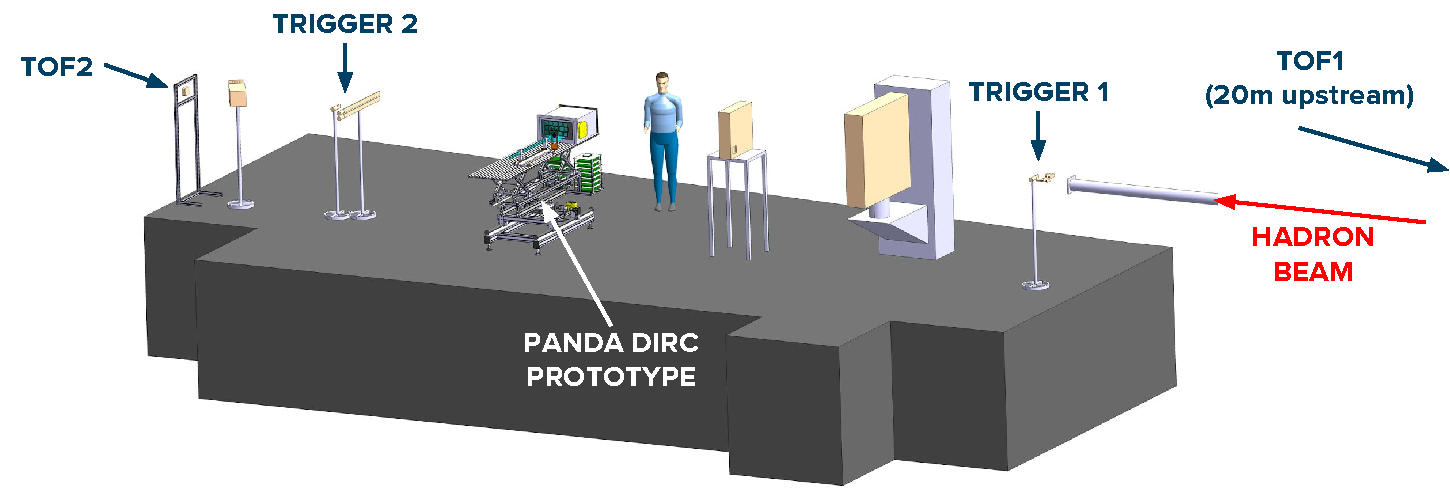
\includegraphics[width=\textwidth]{testbeam_2015.pdf}
	\caption{CAD drawing of the T9 experimental hall with the PANDA DIRC prototype setup. Two time-of-flight (TOF) detectors were separated by 29 m and used for proton/pion separation. Two trigger systems were used for the start and stop times of the readout electronics.}
	\label{fig:testbeam_2015}
\end{figure}

\begin{figure}[ht]
	\centering
	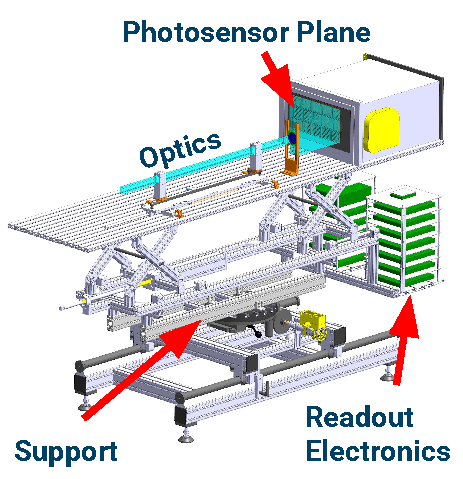
\includegraphics[width=0.6\textwidth]{PANDA_prototype.pdf}
	\caption{CAD drawing of the 2015 PANDA DIRC prototype setup. The radiator, optics, and expansion volume are supported by an aluminum frame that can move in two directions and rotate to allow for measurements at multiple polar angles.}
	\label{fig:PANDA_prototype}
\end{figure}

\begin{figure}[ht]
	\centering
	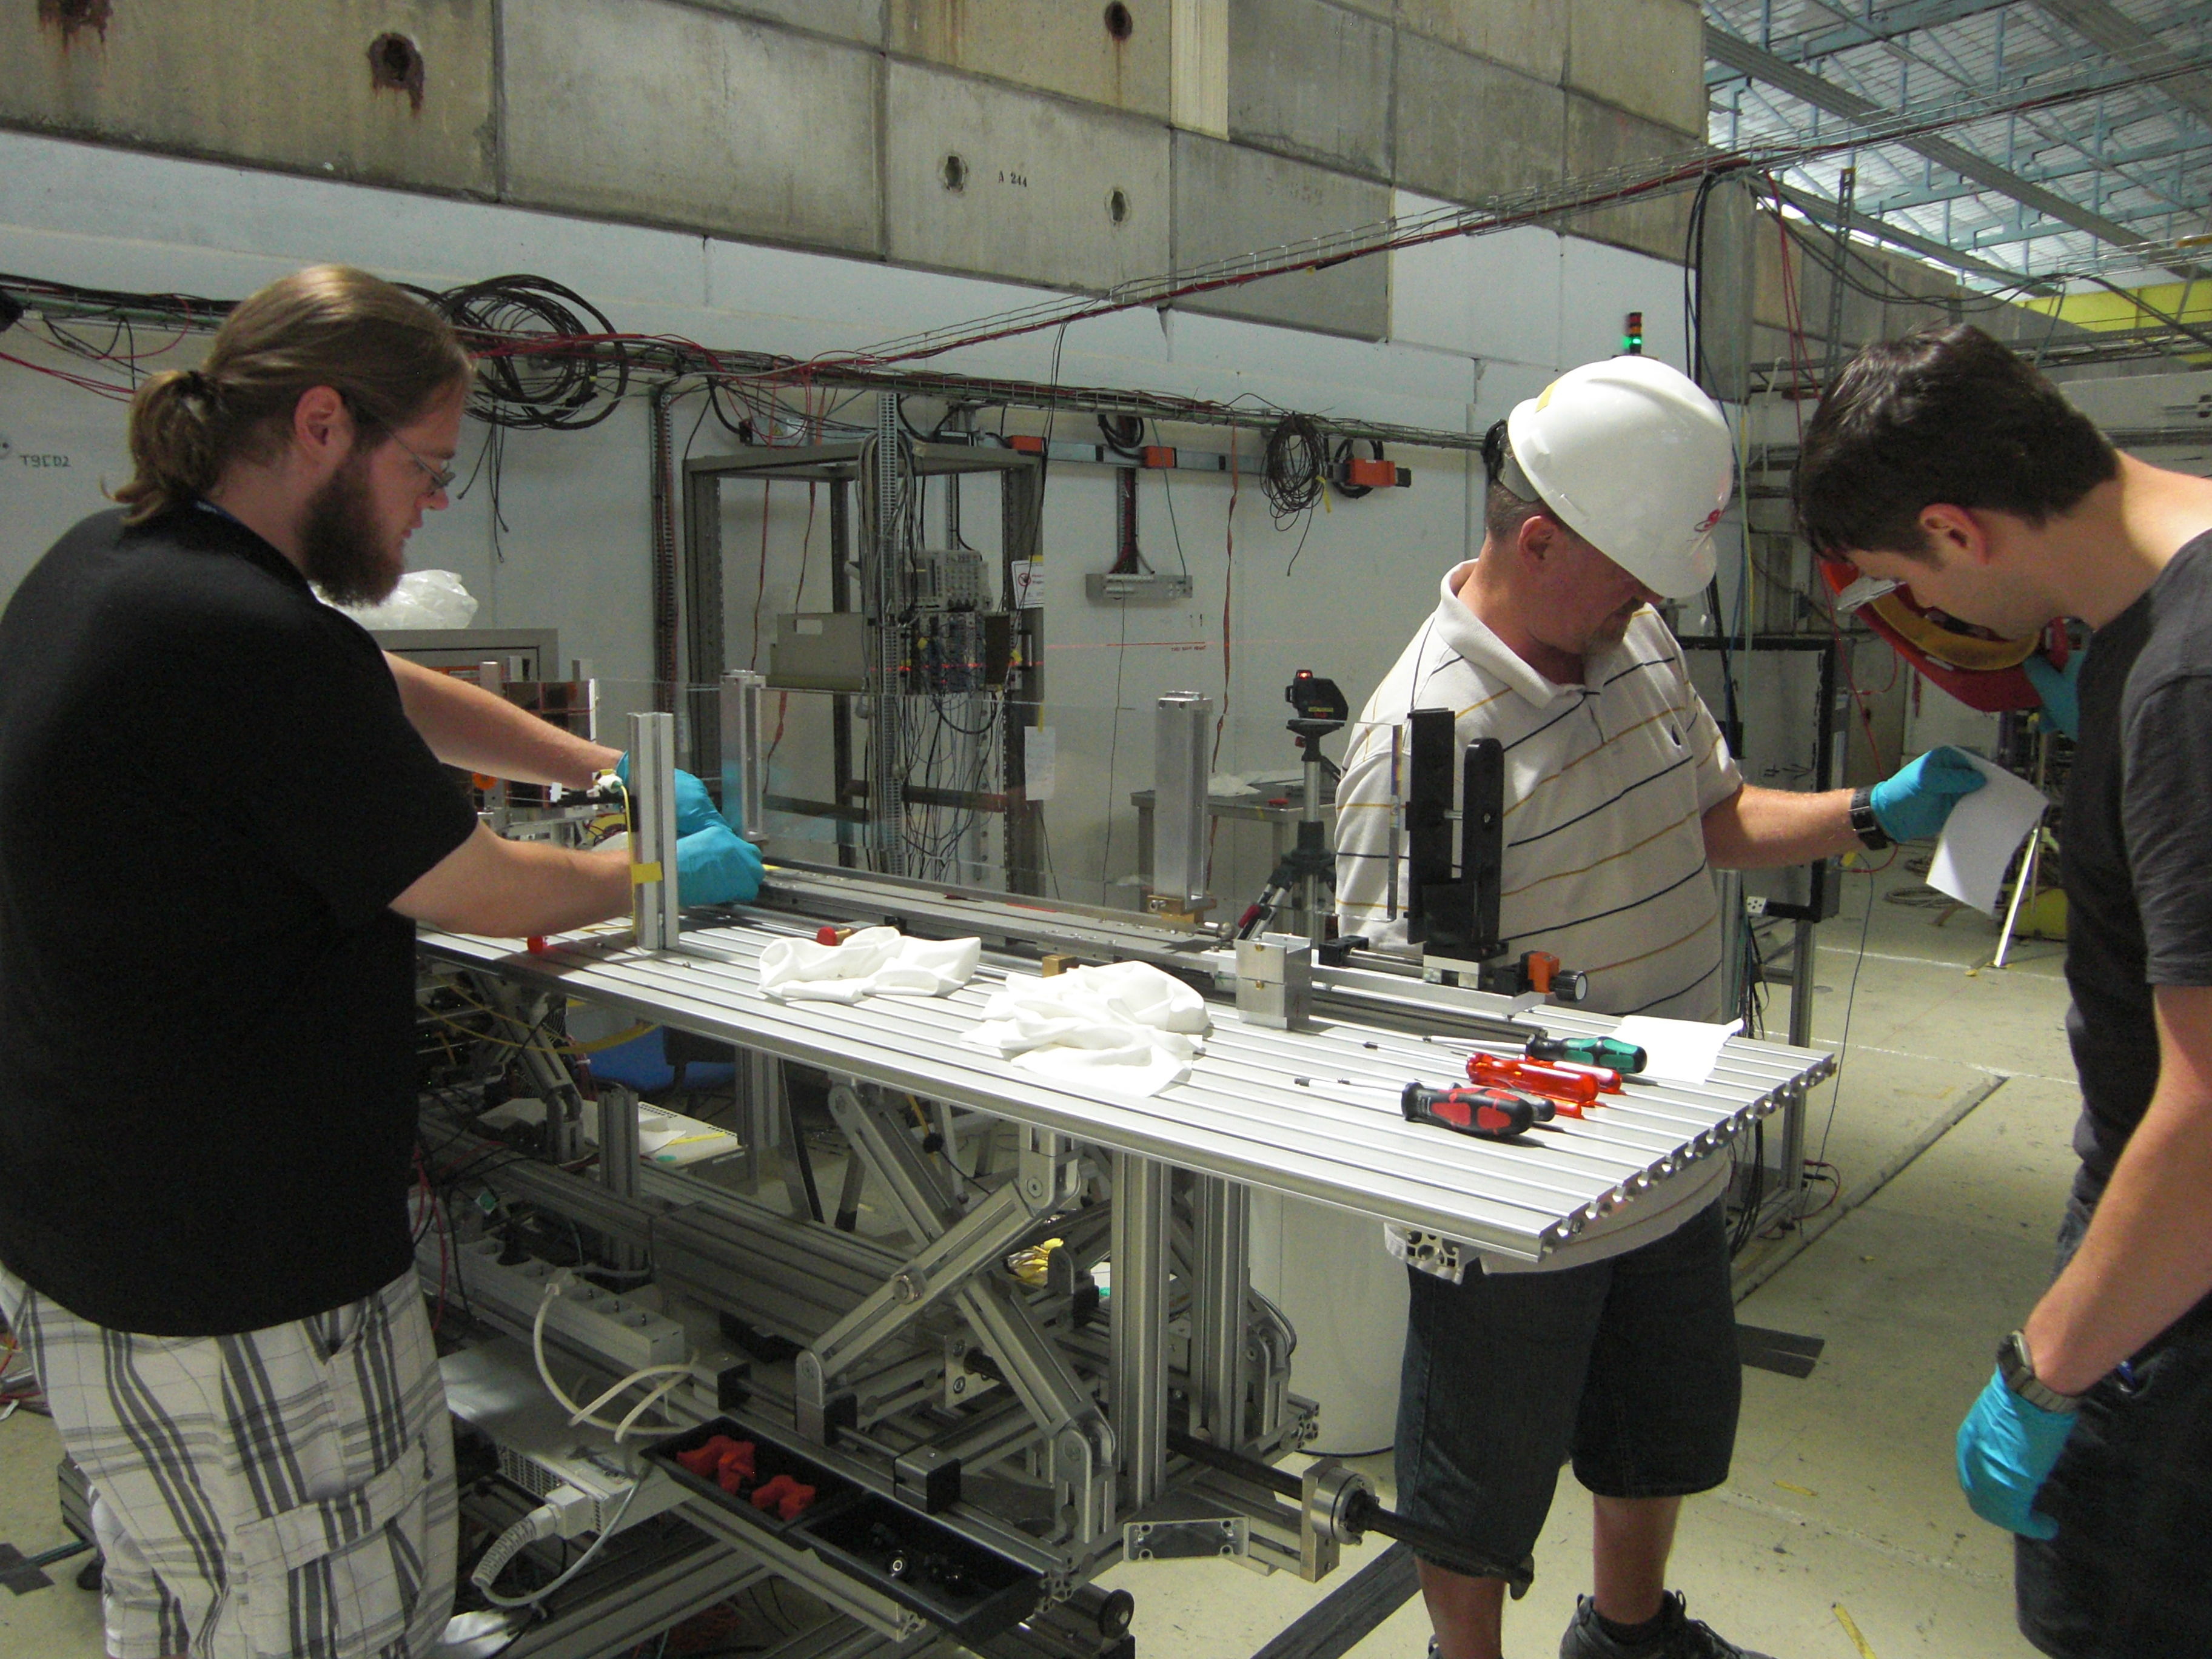
\includegraphics[width=0.8\textwidth]{testbeam_alignment.JPG}
	\caption{Plate radiator being adjusted by micrometer screws using a level laser with both horizontal and vertical beams as a guide. When the light reflected off of the radiator lined up with the incoming beam from the level on the white paper in both directions the radiator was level with the beam.}
	\label{fig:testbeam_alignment}
\end{figure}

\begin{figure}[ht]
	\centering
	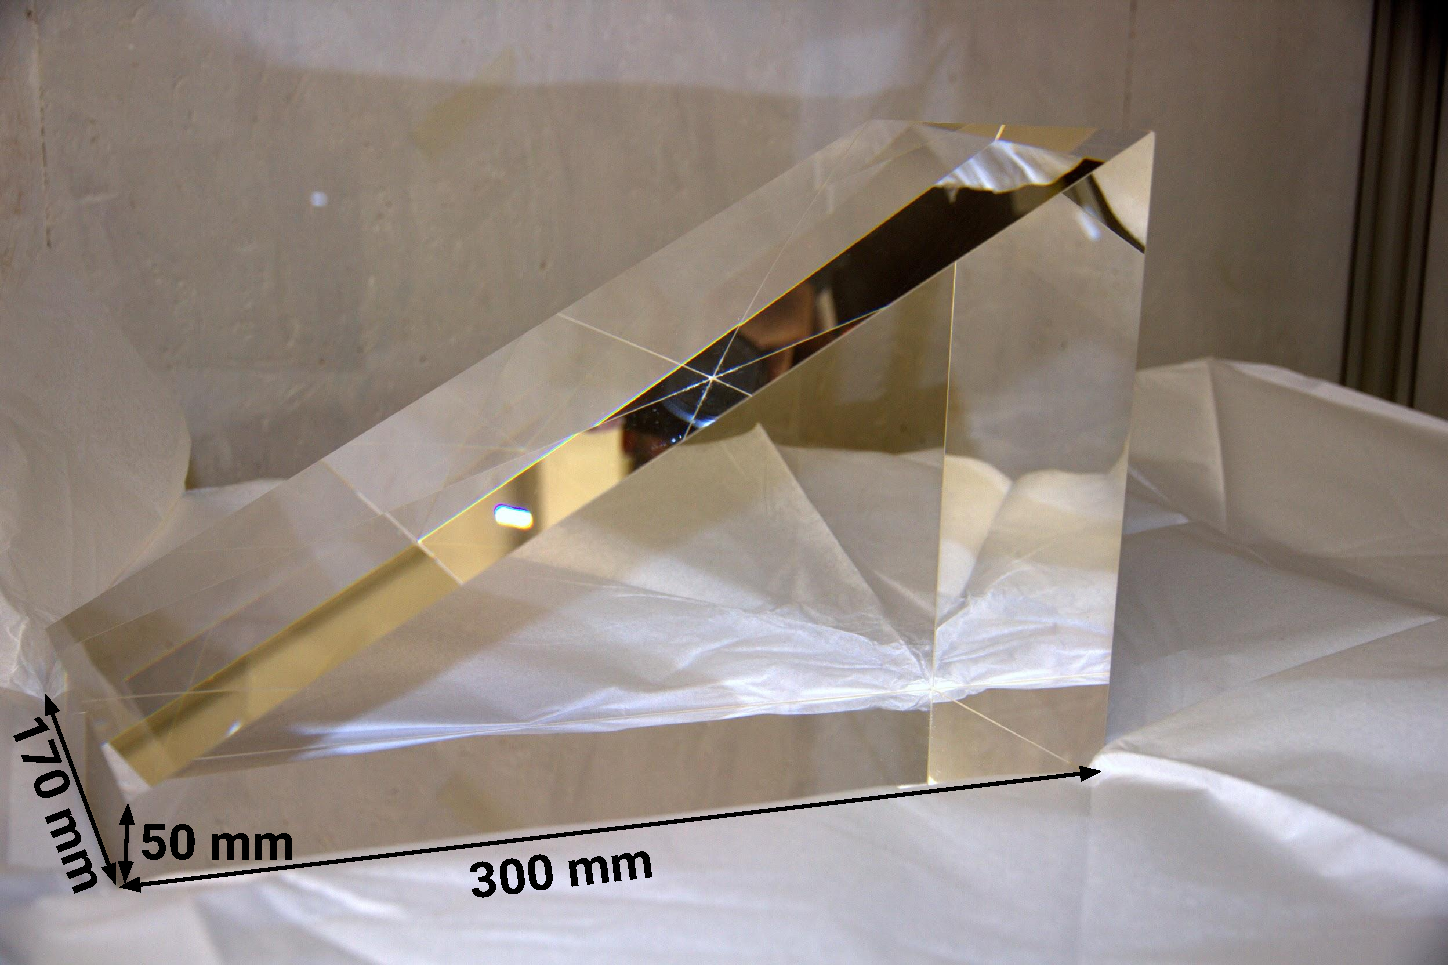
\includegraphics[width=0.7\textwidth]{30-deg-prism.pdf}
	\caption{Picture of the 30$^\circ$ prism expansion volume used in the 2015 test beam.}
	\label{fig:prototype_prism}
\end{figure}


%----------------------------------------------------------------------
%	SIMULATION SECTION
%----------------------------------------------------------------------
\section{Simulated Performance}

%----------------------------------------------------------------------
%	DATA ANALYSIS SECTION
%----------------------------------------------------------------------
\section{Data Analysis}
timing calibration and time walk correction (?)

charge sharing correction

per-MCP thetaC correction

possibility of using simulated background subtraction for data

\subsection{Error Evaluation}